\documentclass[12pt,a4paper,notitlepage,oneside,amsmath,amssymb]{article}
\usepackage{geometry}  % See geometry.pdf to learn the layout options. There are lots.
\geometry{a4paper, margin=1in, noheadfoot} % ... or a4paper or a5paper or ...
\usepackage[utf8]{inputenc}
\usepackage{graphicx}
\graphicspath{{./img/}}
\usepackage{amsmath}
\usepackage{amssymb}
% \usepackage{fontspec}
% \setromanfont{LiHei Pro}
% \XeTeXlinebreaklocale "zh"
% \XeTeXlinebreakskip = 0pt plus 1pt
\usepackage{CJKutf8}
\usepackage{anyfontsize}
\usepackage{caption}
\usepackage{indentfirst}
\usepackage{titlesec}
\usepackage{enumitem}
\usepackage[normalem]{ulem}
\usepackage[most]{tcolorbox}
% \tcbuselibrary{breakable}
% \usepackage{cancel}
\usepackage{xcolor}
% \usepackage[pages=all]{background}
\definecolor{text}{rgb}{0.1, 0.1, 0.1}
\color{black}

\titleformat*{\section}{\large\bfseries}
\titleformat*{\subsection}{\large\bfseries}
\titleformat*{\subsubsection}{\large\bfseries}
\titleformat*{\paragraph}{\large\bfseries}
\titleformat*{\subparagraph}{\large\bfseries}
% \titlespacing*{<command>}{<left>}{<before-sep>}{<after-sep>}
\titlespacing*{\section}{0pt}{15pt}{4pt}


% \setlength{\parindent}{0em}
% \setlength{\parskip}{0.5em}
% \setlength{\columnsep}{0.5cm}
\renewcommand{\baselinestretch}{1.2} % scales the default interline space to 1.5 its default value.

% \setlist[itemize]{topsep=2pt, itemsep=0.2ex, partopsep=0ex, parsep=0ex, nosep, leftmargin=3ex,
% labelindent=1ex, labelwidth=1ex}
% \setlist[enumerate]{topsep=2pt, itemsep=0.2ex, partopsep=0.5ex, parsep=0.2ex, nosep,
%     labelindent=2ex, labelwidth=2ex}

\begin{document}
\begin{CJK*}{UTF8}{bkai}

\CJKtilde{}
\CJKindent{}
\title{\vspace{-10ex}DIP HW3 Report}
\author{R07922036~邱能賢}
\date{\vspace{-1ex}\today}

\maketitle

\vspace{-5ex}

\section*{Problem 1: Morphological Processing}

\begin{enumerate}[label=(\alph*)]
	\item Perform boundary extraction on \(I_1\) to extract the objects’ boundaries and output the result as an image \(B\).

	      I tried to extract the boundaries with the following two methods, where \(H\) is the 3-by-3 structuring element:
	      \[\beta_{inner} (I_1)= I_1 - (I_1 \ominus H)\]
	      \[\beta_{outer} (I_1)= (I_1 \oplus H) - I_1\]

	      \begin{figure}[hbt!]
		      \centering
		      \begin{minipage}{.33\textwidth}
			      \centering
			      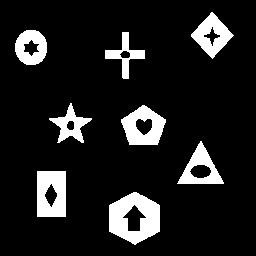
\includegraphics[width=.9\linewidth]{sample1}
			      \caption*{\(I_1\), sample1.raw}
		      \end{minipage}%
		      \begin{minipage}{.33\textwidth}
			      \centering
			      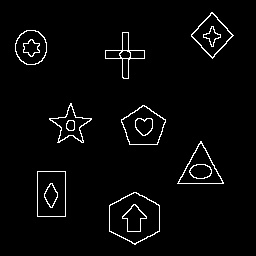
\includegraphics[width=.9\linewidth]{image_B_inner}
			      \caption*{image \(B\) - Inner boundary}
		      \end{minipage}%
		      \begin{minipage}{.33\textwidth}
			      \centering
			      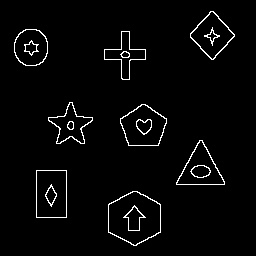
\includegraphics[width=.9\linewidth]{image_B_outer}
			      \caption*{image \(B\) - Outer boundary}
		      \end{minipage}
	      \end{figure}

	\item Perform connected component labeling on \(I_1\) to obtain an image \(C\) where different objects are
	      labeled with different colors.

	      To perform connected component labeling, I iterate the following operation until there is no change in \(G\), starting with \(G_1\) containing only one first-found white pixel:
	      \[G_{i+1} = (G_i \oplus H) \cap I_1\]

	      Mark \(G\) on image \(C\), then erase \(G\) from \(I_1\), and continue with the next connected component.
	      \begin{figure}[hbt!]
		      \centering
		      \begin{minipage}{.4\textwidth}
			      \centering
			      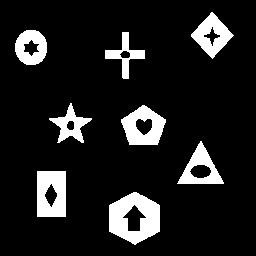
\includegraphics[width=.9\linewidth]{sample1}
			      \caption*{\(I_1\), sample1.raw}
		      \end{minipage}%
		      \begin{minipage}{.4\textwidth}
			      \centering
			      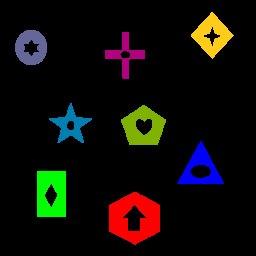
\includegraphics[width=.9\linewidth]{image_C}
			      \caption*{image \(C\)}
		      \end{minipage}
	      \end{figure}

	\item Perform thinning and skeletonizing on \(I_1\) and output the results as image \(D1\) and \(D_2\).


	      Here I used the two-stage algorithm developed by Pratt and Kabir. The operation can be expressed as
	      \[D = I_1 \cap [\bar{M} \cup P]\]
	      where \(M\) and \(P\) are the images generated by the two \(3\times3\) hit-or-miss transformation stages.

	      \begin{figure}[hbt!]
		      \centering
		      \begin{minipage}{.3\textwidth}
			      \centering
			      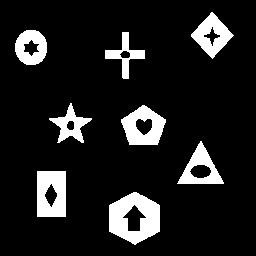
\includegraphics[width=.9\linewidth]{sample1}
			      \caption*{\(I_1\), sample1.raw}
		      \end{minipage}%
		      \begin{minipage}{.3\textwidth}
			      \centering
			      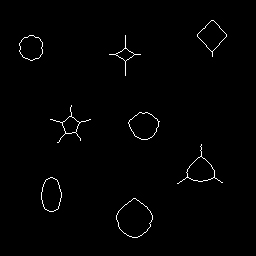
\includegraphics[width=.9\linewidth]{image_D1}
			      \caption*{image \(D_1\)}
		      \end{minipage}%
		      \begin{minipage}{.3\textwidth}
			      \centering
			      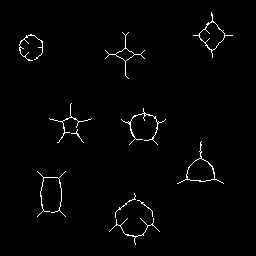
\includegraphics[width=.9\linewidth]{image_D2}
			      \caption*{image \(D_2\)}
		      \end{minipage}
	      \end{figure}

\end{enumerate}

\newpage

\section*{Problem 2: Texture Analysis}
\begin{enumerate}[label=(\alph*)]
\item Perform Law’s method on \(I_2\) to obtain the feature vector of each pixel.

At the second stage, the feature is the energy in a \(19 \times 19\) window.
\begin{figure}[hbt!]
\centering
\begin{minipage}{.24\textwidth}
	\centering
	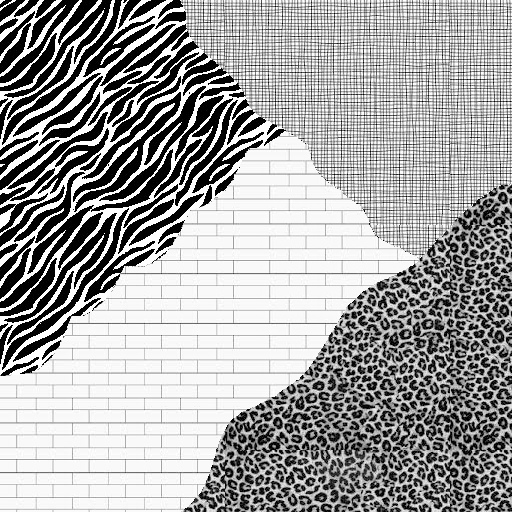
\includegraphics[width=.98\linewidth]{sample2}
	\caption*{\(I_2\), sample2.raw}
\end{minipage}%
\begin{minipage}{.38\textwidth}
\centering
\begingroup
\renewcommand{\arraystretch}{0.4} % Default value: 1
\begin{tabular}[h!]{c@{\hspace{1pt}}c@{\hspace{1pt}}c}
	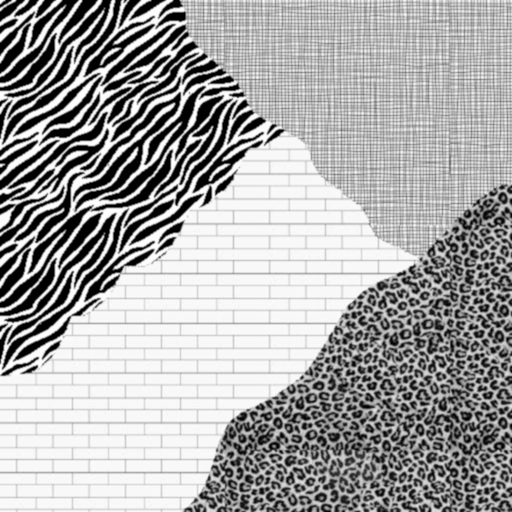
\includegraphics[width=.3\linewidth]{sample2_microstructure1} &
	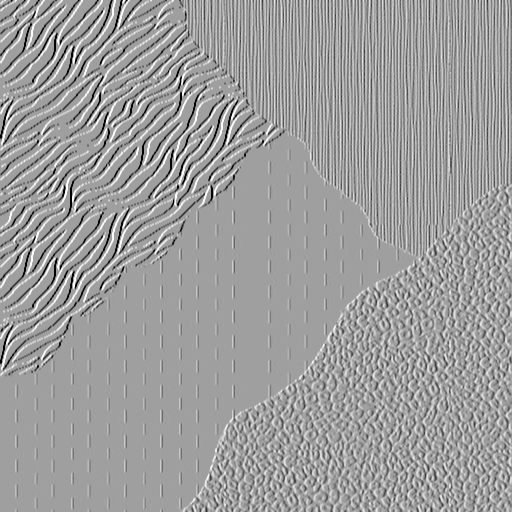
\includegraphics[width=.3\linewidth]{sample2_microstructure2} &
	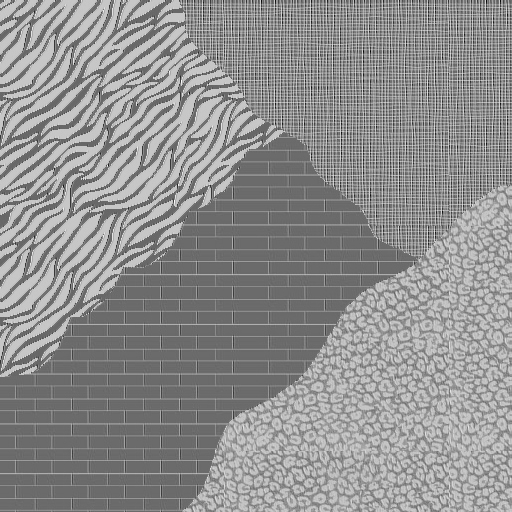
\includegraphics[width=.3\linewidth]{sample2_microstructure3}   \\
	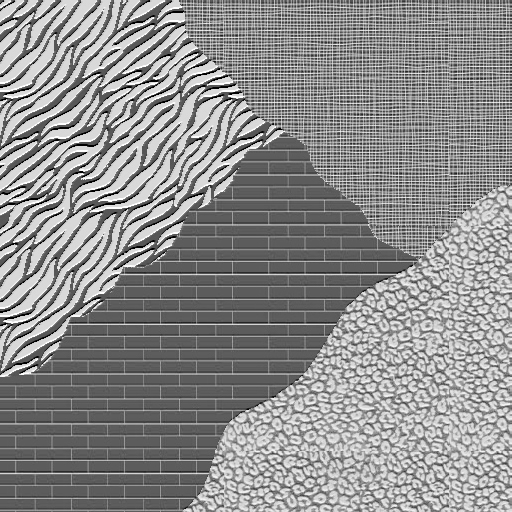
\includegraphics[width=.3\linewidth]{sample2_microstructure4} &
	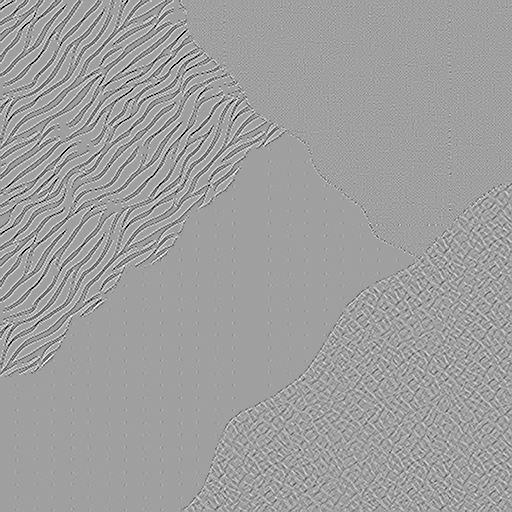
\includegraphics[width=.3\linewidth]{sample2_microstructure5} &
	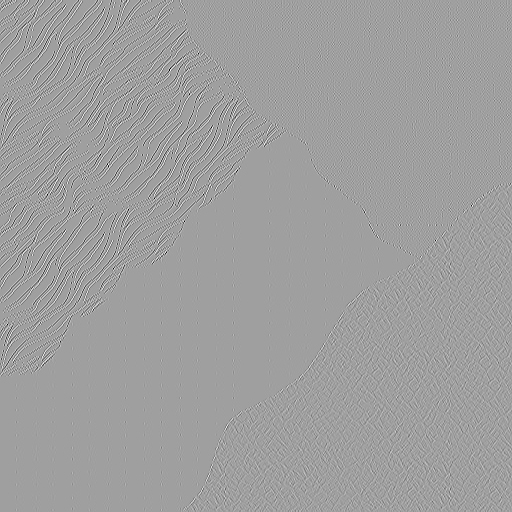
\includegraphics[width=.3\linewidth]{sample2_microstructure6}   \\
	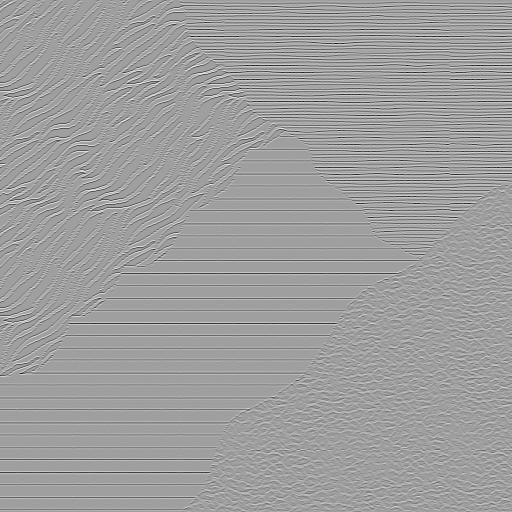
\includegraphics[width=.3\linewidth]{sample2_microstructure7} &
	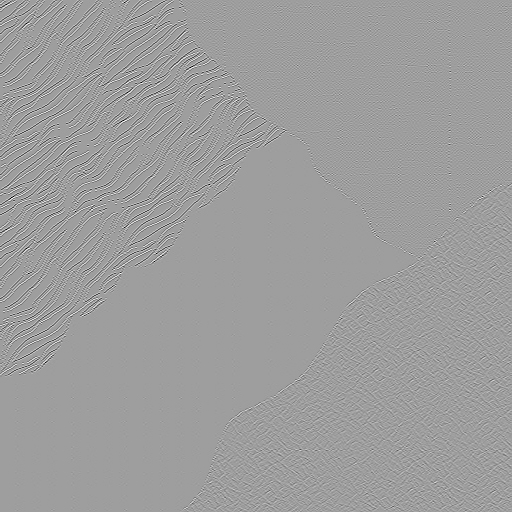
\includegraphics[width=.3\linewidth]{sample2_microstructure8} &
	
\includegraphics[width=.3\linewidth]{sample2_microstructure9}   \\
\end{tabular}
\endgroup
\caption*{9 Micro-structure response}
\end{minipage}%
\begin{minipage}{.38\textwidth}
\centering
\begingroup
\renewcommand{\arraystretch}{0.4} % Default value: 1
\begin{tabular}[h!]{c@{\hspace{1pt}}c@{\hspace{1pt}}c}
	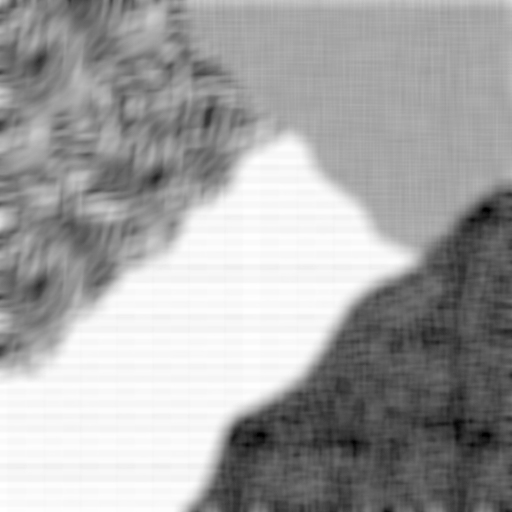
\includegraphics[width=.3\linewidth]{sample2_feature1} &
	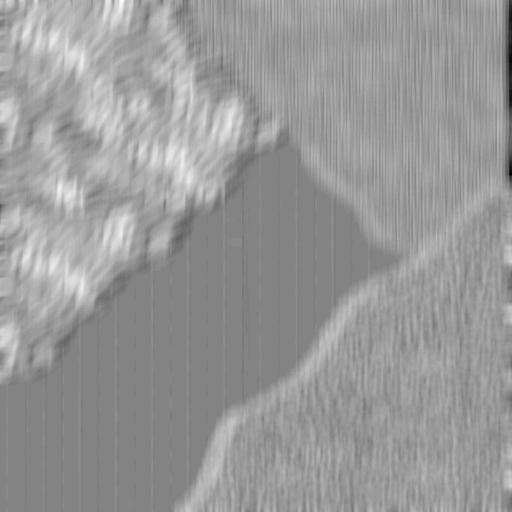
\includegraphics[width=.3\linewidth]{sample2_feature2} &
	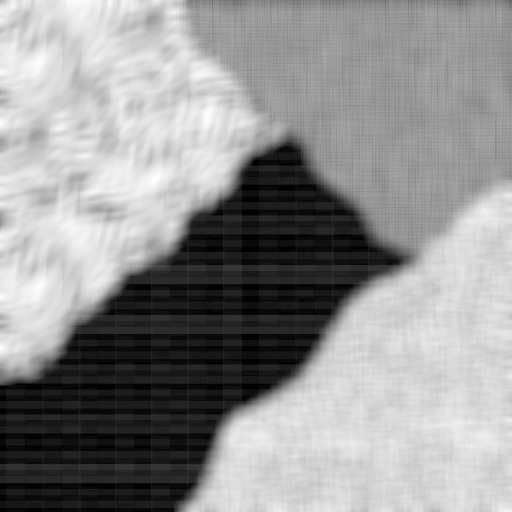
\includegraphics[width=.3\linewidth]{sample2_feature3}   \\
	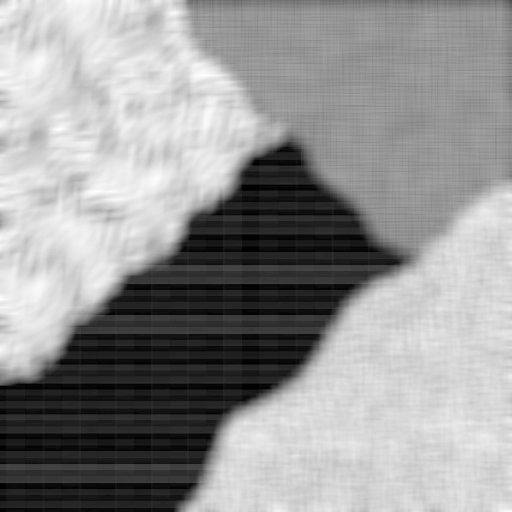
\includegraphics[width=.3\linewidth]{sample2_feature4} &
	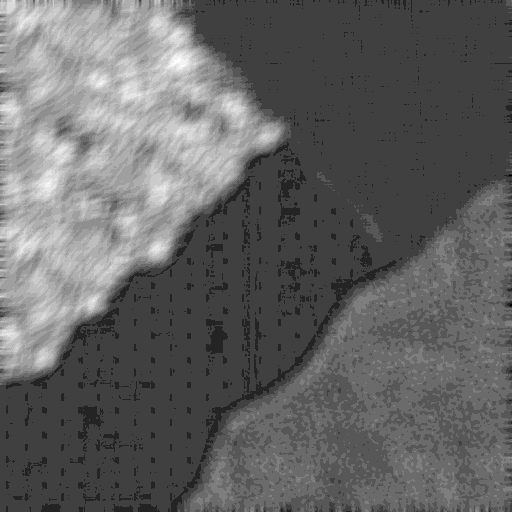
\includegraphics[width=.3\linewidth]{sample2_feature5} &
	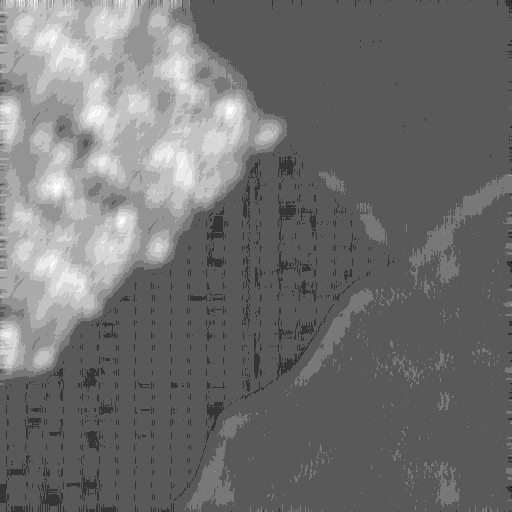
\includegraphics[width=.3\linewidth]{sample2_feature6}   \\
	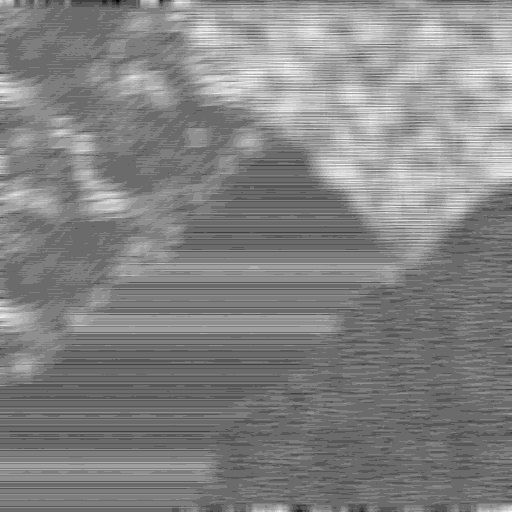
\includegraphics[width=.3\linewidth]{sample2_feature7} &
	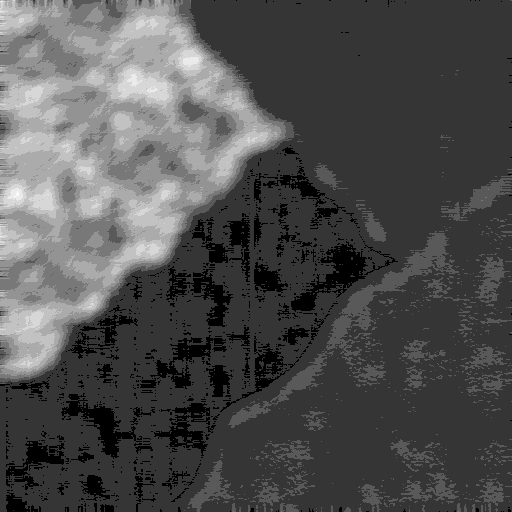
\includegraphics[width=.3\linewidth]{sample2_feature8} &
	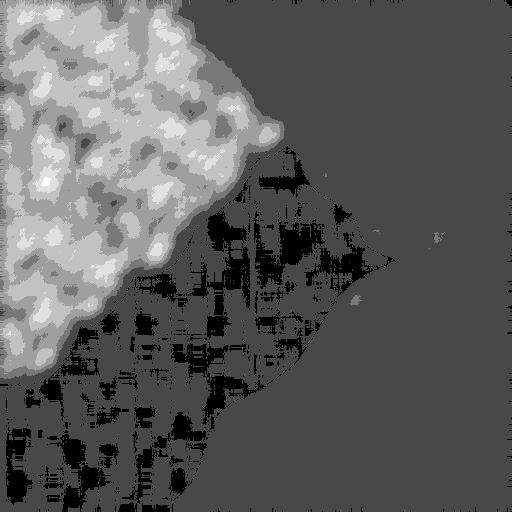
\includegraphics[width=.3\linewidth]{sample2_feature9}   \\
\end{tabular}
\endgroup
\caption*{Feature vectors (Energy)}
\end{minipage}
\end{figure}

\item Use k-means to classify each pixel and label same kind of texture with same gray-level intensity and output the result as image \(E\).

	The following is the resulting image \(E\) using k-means to classify each pixel. The centroid gets stable after 8 iterations. As the image shows, there are lots of holes in the top left texture, also the classification is poor at texture boundaries. When the energy window increases, the holes become less but the mis-classified boundary gets wider.

	\begin{figure}[hbt!]
		\centering
		\begin{minipage}{.4\textwidth}
			\centering
			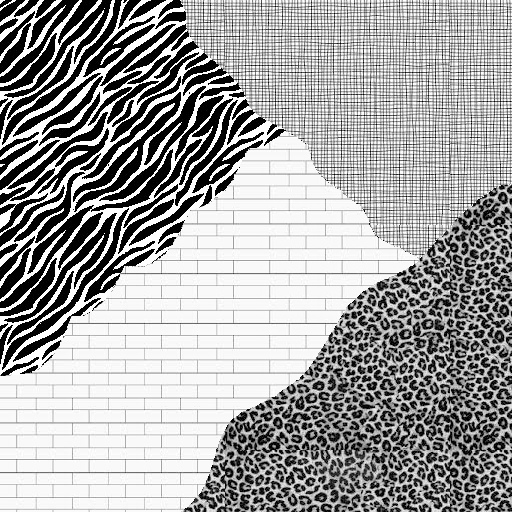
\includegraphics[width=.7\linewidth]{sample2}
			\caption*{\(I_2\), sample2.raw}
		\end{minipage}%
		\begin{minipage}{.4\textwidth}
			\centering
			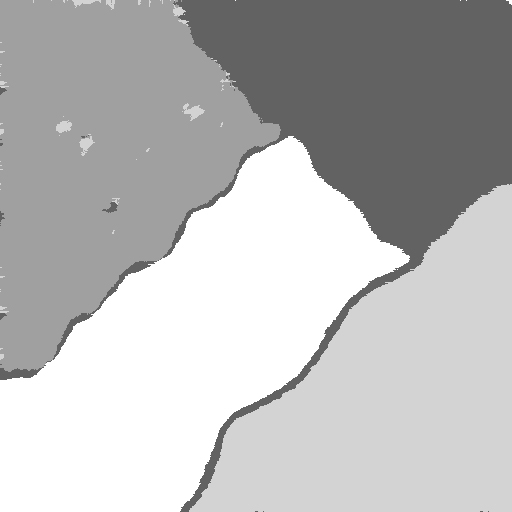
\includegraphics[width=.7\linewidth]{image_E}
			\caption*{Image \(E\)}
		\end{minipage}
	\end{figure}

	So, I use the following method to improve the texture segmentation.

	\begin{enumerate}
		\item First extract the 4 texture to its own binarized image.

	\begin{figure}[hbt!]
		\centering
		\begin{minipage}{.25\textwidth}
			\centering
			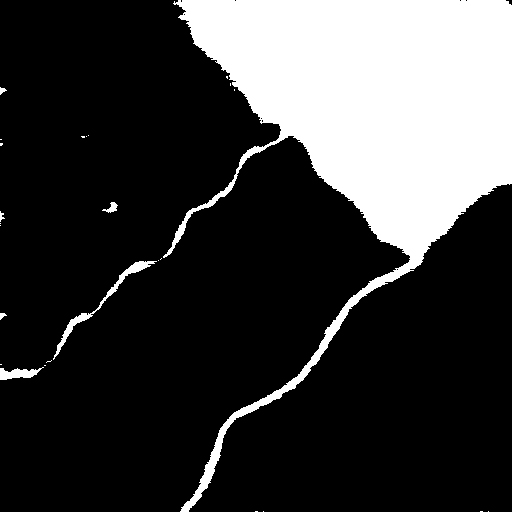
\includegraphics[width=.9\linewidth]{sample2_texture1_0}
			\caption*{Texture 1.}
		\end{minipage}%
		\begin{minipage}{.25\textwidth}
			\centering
			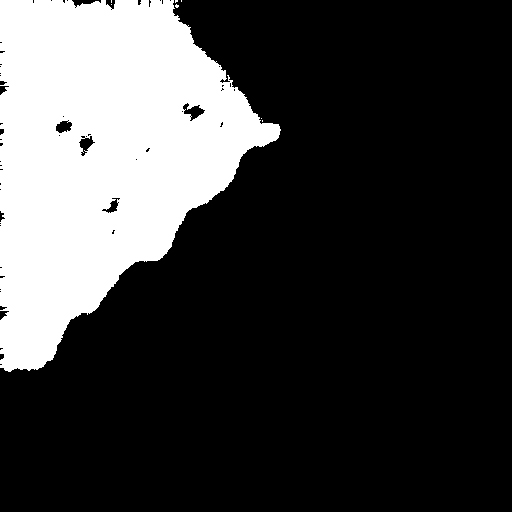
\includegraphics[width=.9\linewidth]{sample2_texture2_0}
			\caption*{Texture 2.}
		\end{minipage}%
		\begin{minipage}{.25\textwidth}
			\centering
			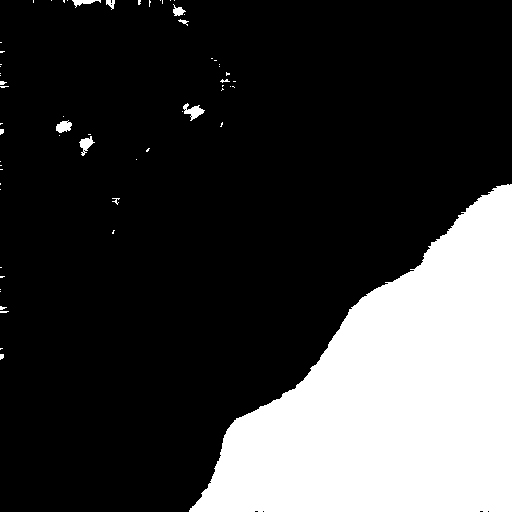
\includegraphics[width=.9\linewidth]{sample2_texture3_0}
			\caption*{Texture 3.}
		\end{minipage}%
		\begin{minipage}{.25\textwidth}
			\centering
			
\includegraphics[width=.9\linewidth]{sample2_texture4_0}
			\caption*{Texture 4.}
		\end{minipage}
	\end{figure}

	\item Perform the close operator followed by the open operator on each texture.

	\begin{figure}[hbt!]
		\centering
		\begin{minipage}{.25\textwidth}
			\centering
			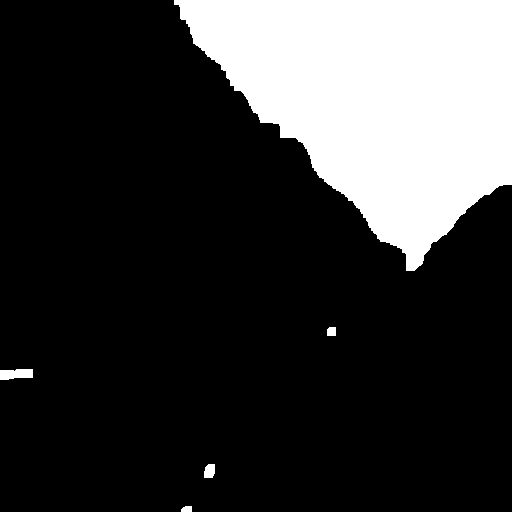
\includegraphics[width=.9\linewidth]{sample2_texture1_1}
			\caption*{Texture 1.}
		\end{minipage}%
		\begin{minipage}{.25\textwidth}
			\centering
			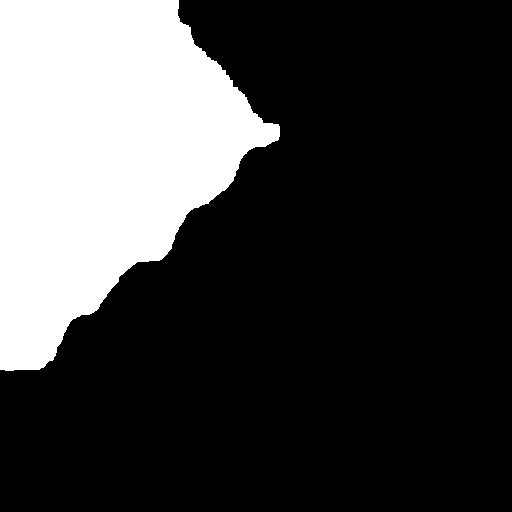
\includegraphics[width=.9\linewidth]{sample2_texture2_1}
			\caption*{Texture 2.}
		\end{minipage}%
		\begin{minipage}{.25\textwidth}
			\centering
			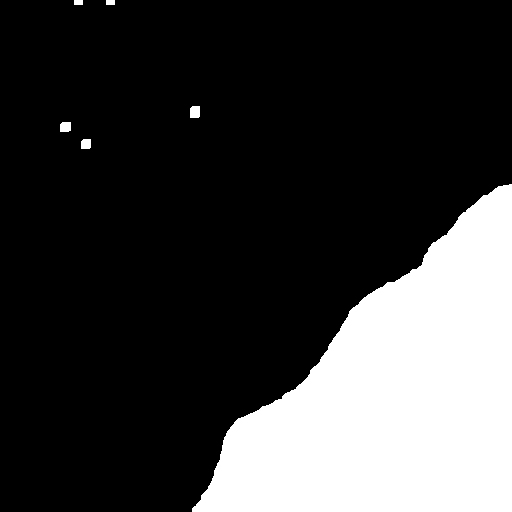
\includegraphics[width=.9\linewidth]{sample2_texture3_1}
			\caption*{Texture 3.}
		\end{minipage}%
		\begin{minipage}{.25\textwidth}
			\centering
			
\includegraphics[width=.9\linewidth]{sample2_texture4_1}
			\caption*{Texture 4.}
		\end{minipage}
	\end{figure}

	\item Perform connected component labeling and remove components whose area is less than 1000 pixels.

	\begin{figure}[hbt!]
		\centering
		\begin{minipage}{.25\textwidth}
			\centering
			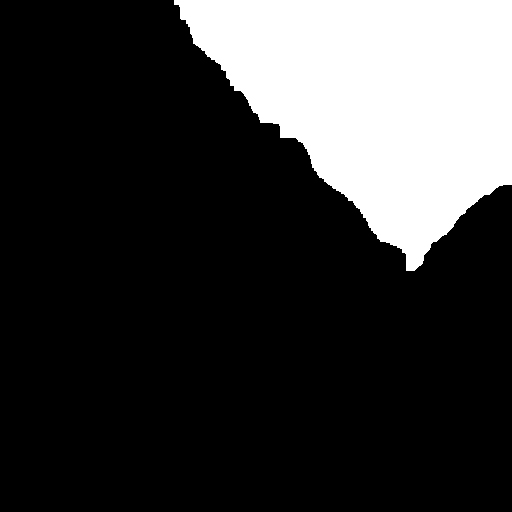
\includegraphics[width=.9\linewidth]{sample2_texture1}
			\caption*{Texture 1.}
		\end{minipage}%
		\begin{minipage}{.25\textwidth}
			\centering
			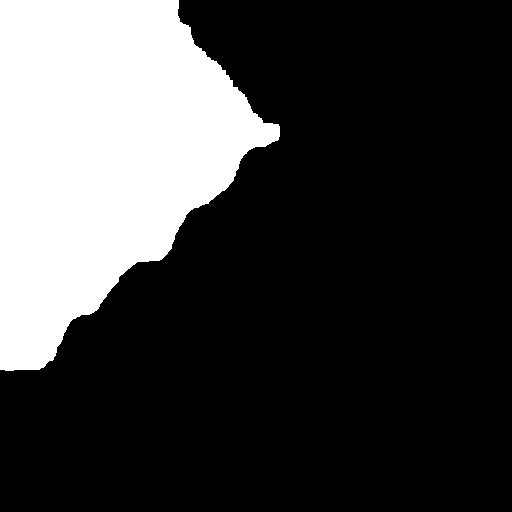
\includegraphics[width=.9\linewidth]{sample2_texture2}
			\caption*{Texture 2.}
		\end{minipage}%
		\begin{minipage}{.25\textwidth}
			\centering
			
\includegraphics[width=.9\linewidth]{sample2_texture3}
			\caption*{Texture 3.}
		\end{minipage}%
		\begin{minipage}{.25\textwidth}
			\centering
			
\includegraphics[width=.9\linewidth]{sample2_texture4}
			\caption*{Texture 4.}
		\end{minipage}
	\end{figure}

	\end{enumerate}

	\newpage
	Here is the merged image:

	\begin{figure}[hbt!]
		\centering
		\begin{minipage}{.4\textwidth}
			\centering
			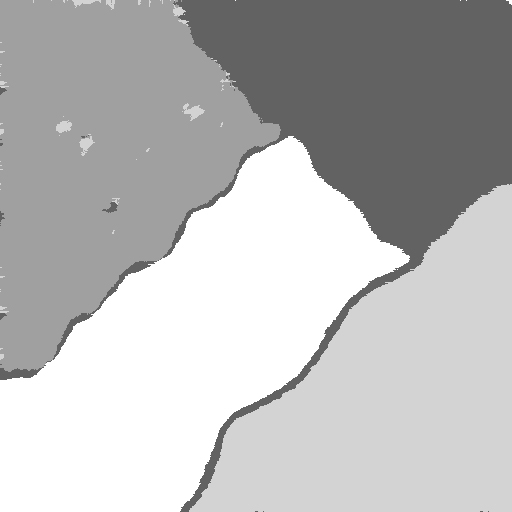
\includegraphics[width=.6\linewidth]{image_E}
			\caption*{Original image \(E\).}
		\end{minipage}%
		\begin{minipage}{.4\textwidth}
			\centering
			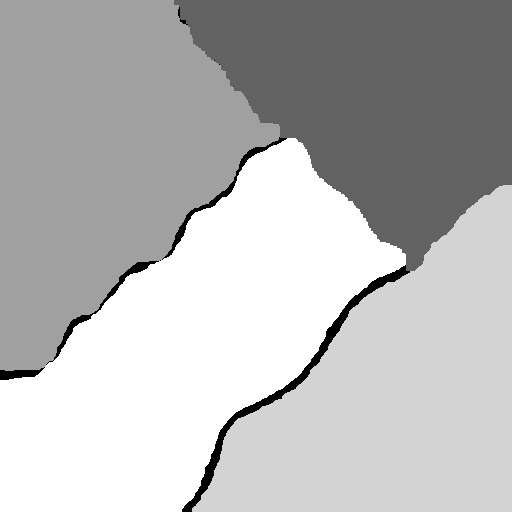
\includegraphics[width=.6\linewidth]{image_E2}
			\caption*{Optimized image \(E\).}
		\end{minipage}
	\end{figure}

There are still gaps at texture boundaries, so I assign unclassified pixels to its nearest texture to fill the gap.

\begin{figure}[hbt!]
	\centering
	\begin{minipage}{.4\textwidth}
		\centering
		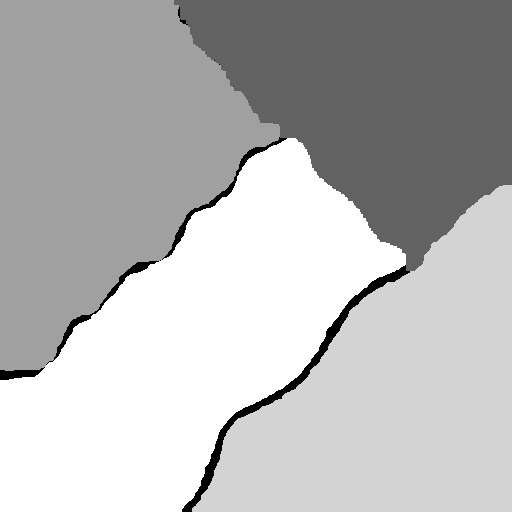
\includegraphics[width=.6\linewidth]{image_E2}
		\caption*{Optimized image \(E\).}
	\end{minipage}%
	\begin{minipage}{.4\textwidth}
		\centering
		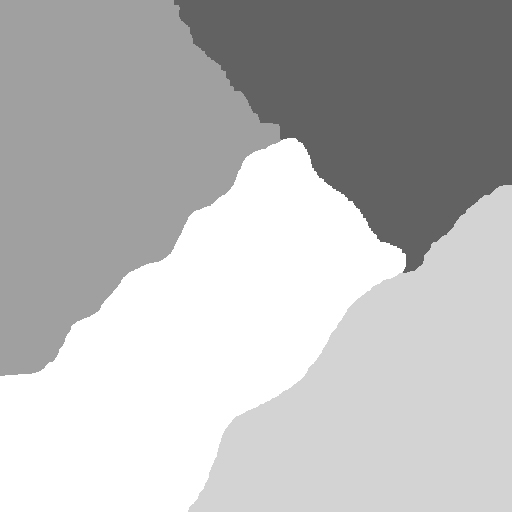
\includegraphics[width=.6\linewidth]{image_E3}
		\caption*{Image \(E\) after gap filling.}
	\end{minipage}
\end{figure}

\newpage

\item Based on \(E\), try to generate another texture image by exchanging the types of different texture patterns as image \(G\).

I tried implementing the image quilting \cite{Efros01} algorithm. I cropped an \(84 \times 84\) block from \(I_2\) and generated the 4 texture image.


\begin{figure}[hbt!]
	\centering
	\begin{minipage}{.25\textwidth}
		\centering
		
\includegraphics[width=.85\linewidth]{synthesized_texture1}
		\caption*{Texture 1.}
	\end{minipage}%
	\begin{minipage}{.25\textwidth}
		\centering
		
\includegraphics[width=.85\linewidth]{synthesized_texture2}
		\caption*{Texture 2.}
	\end{minipage}%
	\begin{minipage}{.25\textwidth}
		\centering
		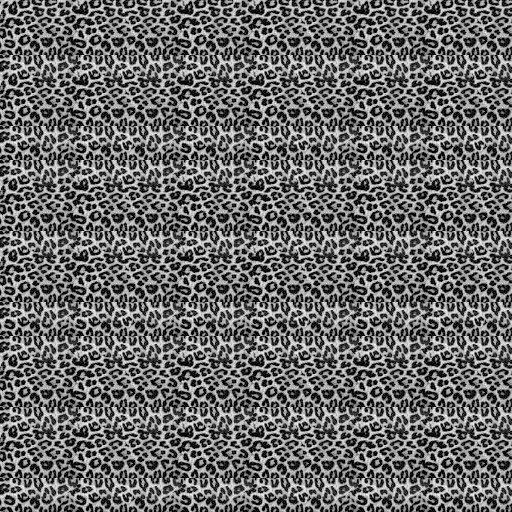
\includegraphics[width=.85\linewidth]{synthesized_texture3}
		\caption*{Texture 3.}
	\end{minipage}%
	\begin{minipage}{.25\textwidth}
		\centering
		
\includegraphics[width=.85\linewidth]{synthesized_texture4}
		\caption*{Texture 4.}
	\end{minipage}
\end{figure}

Then use the segmentation from image \(E\) to merge the textures in different orders.

\begin{figure}[hbt!]
	\centering
	\begin{minipage}{.35\textwidth}
		\centering
		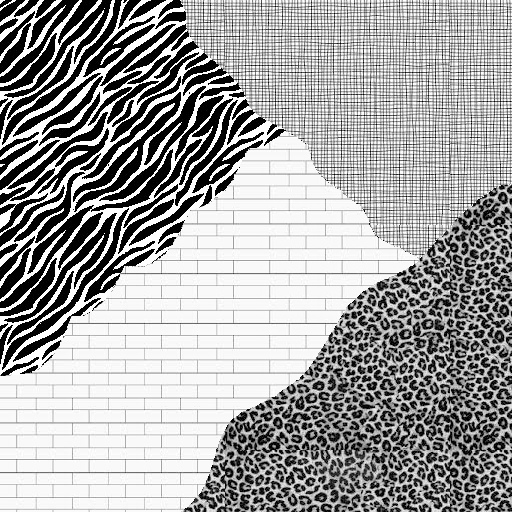
\includegraphics[width=.7\linewidth]{sample2}
		\caption*{\(I_2\), sample2.raw}
	\end{minipage}%
	\begin{minipage}{.35\textwidth}
		\centering
		\includegraphics[width=.7\linewidth]{image_G}
		\caption*{Image \(G\)}
	\end{minipage}
\end{figure}

\end{enumerate}


\begin{thebibliography}{9}
	\bibitem{Efros01}
``Image Quilting.`` Efros and Freeman. SIGGRAPH 2001
\end{thebibliography}

\clearpage

\end{CJK*}
\end{document}
